\chapter{Rhythmic Similarity}\label{rhythmsimc}

\section{Cross Correlation}

- simple approach using only onset and beat features extracted with librosa
- cross correlation of 2 songs

dependent on beat extraction and onset detection algorithms

\section{fluctuation patterns}

\section{Tempo Estimation}

\section{Beat and Tatum Estimation}

%==============================================================

\chapter{Pitch estimation/ Chroma Features}\label{melsimc}

\textit{TODO: 
pros and cons\\
bring all songs to standard key \\
usage (cover song identification)\\
text based (levenshtein distance)\\
different representations of melody (Chroma Features)\\}

\section{Pitch Curve}

As presented in section \ref{midiest} there are tools for pitch curve extraction of the main melody line. However in polyphonic music these kind of algorithms struggle to get reasonable results, even in popcultural music. In musical genres like Metal it gets even worse. 


\section{MIDI representation}


\section{Graph representation}

\section{Chroma Features}

Chroma Features as described in section \ref{featsec} are a good and low dimensional way to describe the melodic features of a song. 
The reduction of dimensionality however comes with a loss of information, especially what octaves the notes are played in. 

\begin{figure}[htbp]
	\centering
	\framebox{\parbox{1\textwidth}{ 
			\begin{subfigure}{.495\textwidth}
				\centering 
				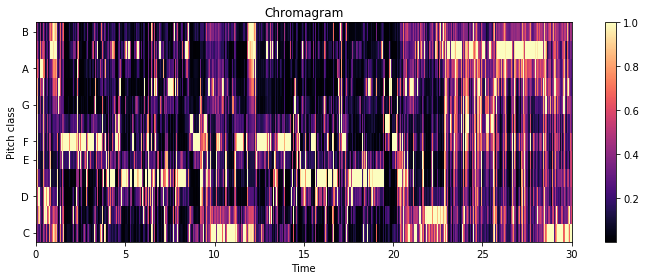
\includegraphics[scale=0.3]{Images/Chroma/sia.png}
				\caption{Chroma Features of unfiltered audio}
				\label{sia}
			\end{subfigure}%
			\begin{subfigure}{.495\textwidth}
				\centering
				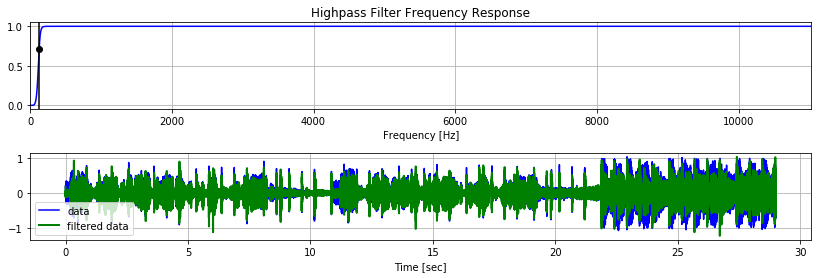
\includegraphics[scale=0.3]{Images/Chroma/siahp.png}
				\caption{Highpassfilter}
				\label{siahp}
			\end{subfigure}%
			
			\begin{subfigure}{.495\textwidth}
				\centering    
				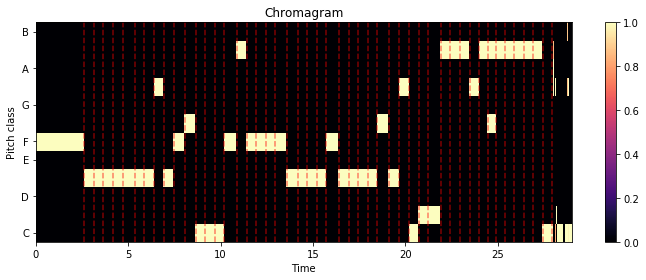
\includegraphics[scale=0.3]{Images/Chroma/siaunfiltered.png}
				\caption{Beat aligned of unfiltered audio}
				\label{siaub}
			\end{subfigure}
			\begin{subfigure}{.495\textwidth}
				\centering     
				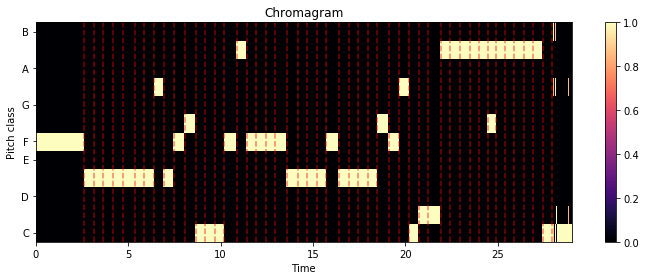
\includegraphics[scale=0.3]{Images/Chroma/siafiltered.png}
				\caption{Beat aligned of filtered audio}
				\label{siafb}
			\end{subfigure}%			
	}}
	\caption{Sia Features}
	\label{fig:sia1}
\end{figure}


\begin{figure}[htbp]
	\centering
	\framebox{\parbox{1\textwidth}{ 
			\begin{subfigure}{.495\textwidth}
				\centering 
				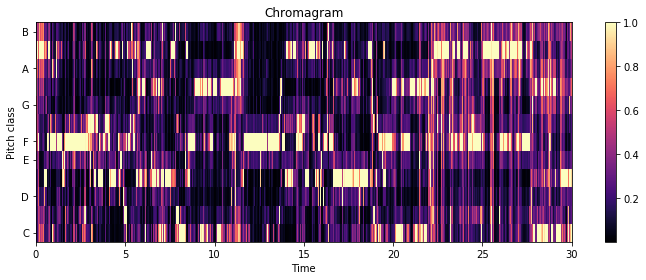
\includegraphics[scale=0.3]{Images/Chroma/pvris.png}
				\caption{Chroma Features of unfiltered audio}
				\label{pv}
			\end{subfigure}%
			\begin{subfigure}{.495\textwidth}
				\centering
				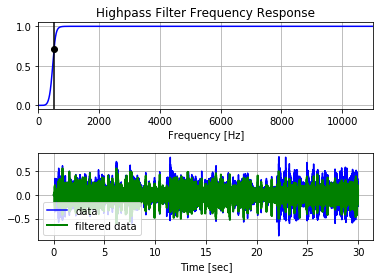
\includegraphics[scale=0.3]{Images/Chroma/pvrishp.png}
				\caption{Highpassfilter}
				\label{pvhp}
			\end{subfigure}%
			
			\begin{subfigure}{.495\textwidth}
				\centering    
				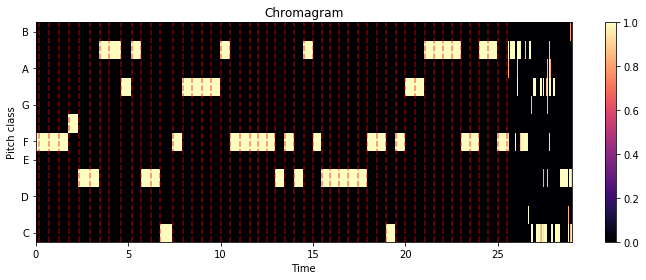
\includegraphics[scale=0.3]{Images/Chroma/pvrisunfiltered.png}
				\caption{Beat aligned of unfiltered audio}
				\label{pvub}
			\end{subfigure}		
			\begin{subfigure}{.495\textwidth}
				\centering     
				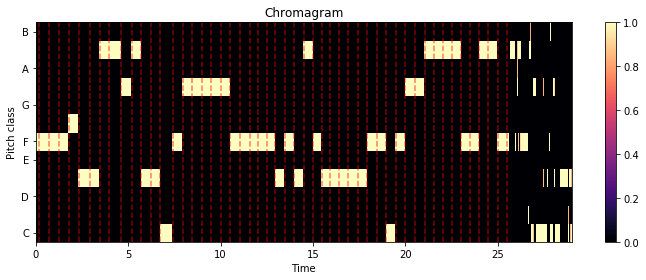
\includegraphics[scale=0.3]{Images/Chroma/pvrisfiltered.png}
				\caption{Beat aligned of filtered audio}
				\label{pvfb}
			\end{subfigure}%	
	}}
	\caption{Pvris Features}
	\label{fig:pvris1}
\end{figure}

\subsection{Bandpass filter}

\subsection{Key invariance}



\subsection{Beat alignment}



\subsection{Validation}

A good measure for the efficiency of a melodic similarity algorithm is the ability to find cover songs. 


